\subsection{A real diffusion model fabricates recoverable morphology}
The strongest test is non-circular: on the certified-unrecoverable subspace
$\rho(\widehat{\bm L},\bm L)\!\approx\!0$ for \emph{any} sampler, so a low $\rho$ there
measures the definition, not fabrication. We therefore build a \emph{held-out oracle}: a
supervised ridge predictor (fit on train folds) whose held-out correlation
$\rho_{\rm oracle}$ is a \emph{lower bound} on recoverability: $\rho_{\rm oracle}{>}0$
\emph{proves} that this much of an unobserved lead's non-dipolar residual is recoverable
from the observed leads (a simple linear map attains it out of sample). For
$S{=}\{$I,II,V1,V3,V5$\}\!\to\!\{$V2,V4,V6$\}$ (precordial interpolation) the non-dipolar
residual is provably recoverable across the diagnostic segments (aggregate
$\rho_{\rm oracle}{=}\OraAgg$ over QRS/ST/T $\times\{$V2,V4,V6$\}$; $\OraQRS$ for QRS
alone; Band~A); the limb-6 control is lower but still nonzero ($\rho_{\rm oracle}{=}
\negOra$), which we use to check the deficit does not fire spuriously. We train a
conditional 1-D DDPM (classifier-free guidance, RePaint measurement replacement) on NORM
PTB-XL and score held-out NORM reconstructions with the certificate (Fig.~\ref{fig:gpu};
all quantities below are averaged over QRS/ST/T $\times\{$V2,V4,V6$\}$).

Two comparisons are needed to avoid a mean-vs-sample confound: the diffusion
\emph{posterior mean} ($K$-sample average, variance-free) and a single deployed draw.
At the honest end ($w{=}1$) the posterior mean \emph{matches} the oracle
($\Delta\rho{=}\dRhoMeanOne$): the model is competent and Band~A is genuinely
recoverable. As the guidance scale $w$ rises the mean output sharpens toward
population-typical morphology and develops a \emph{growing recoverability deficit}
$\Delta\rho{=}\rho_{\rm oracle}{-}\rho_{\rm mean}$, reaching $\dRhoMeanMax$ at
$w{=}\wmaxval$ --- a genuine distributional effect, not single-sample variance. A single
deployed draw carries an \emph{additional} sampling-variance deficit (total
$\dRhoSampMax$). Crucially the same outputs stay faithful on the recoverable
\emph{dipole} subspace ($\rho_{\rm recoverable}{=}\RhoRec$): the model is competent, not
broken, and RMSE stays in a narrow, non-monotone band ($\rmseLo$--$\rmseHi$\,mV) that
does \emph{not} track the deficit --- which is therefore invisible to a scalar and
localized only by the certificate. On the limb-6 control, where the linear reference is
lower but nonzero ($\negOra$), the diffusion still matches or exceeds it and the deficit
stays negative ($\Delta\rho{=}\negQRSdRho$, QRS): a positive $\Delta\rho$ flags a genuine
\emph{failure to recover} provable content, not the mere act of raising guidance.

\begin{figure}[t]
  \centering
  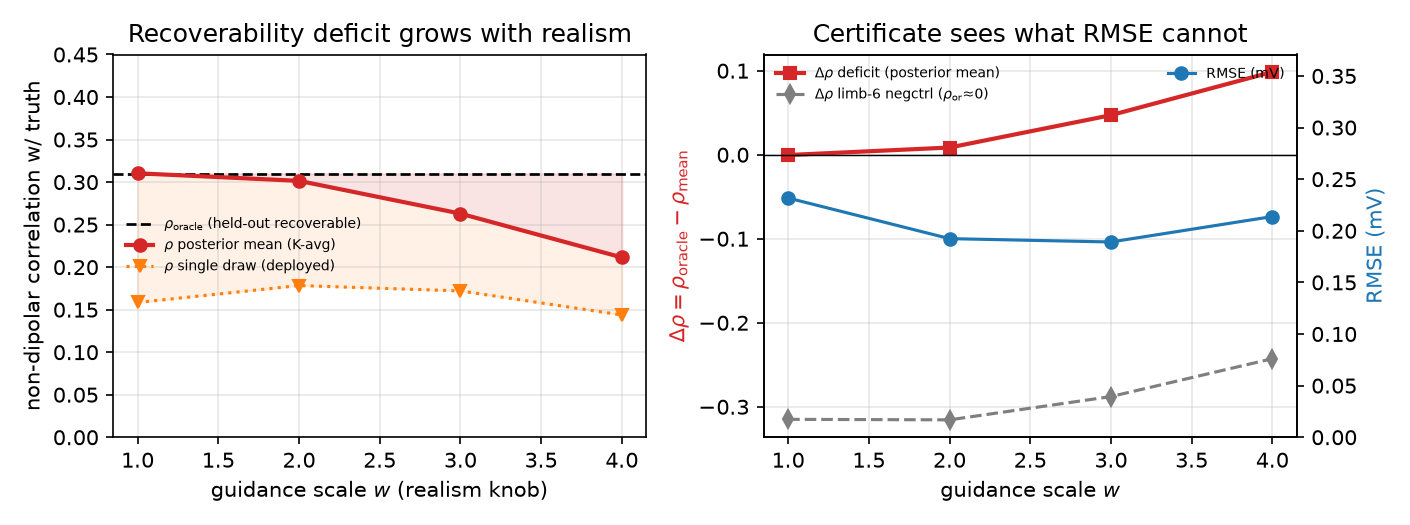
\includegraphics[width=\linewidth]{../results/gpu_diffusion_frontier.png}
  \caption{Conditional DDPM, $S{=}\{$I,II,V1,V3,V5$\}\!\to\!\{$V2,V4,V6$\}$, held-out
  NORM PTB-XL. \emph{Left}: the posterior mean tracks the held-out recoverable reference
  $\rho_{\rm oracle}$ at low guidance and pulls away as $w$ rises (red band = a genuine
  recoverability deficit); a single deployed draw sits a fixed sampling-variance band
  below (orange). \emph{Right}: the deficit $\Delta\rho$ grows monotonically with the
  realism knob while RMSE stays in a narrow non-monotone band, and the limb-6 control
  shows no positive deficit --- the certificate sees, and localizes, what a scalar
  cannot. All curves average QRS/ST/T $\times\{$V2,V4,V6$\}$.}
  \label{fig:gpu}
\end{figure}
